\documentclass[tikz,border=8pt]{standalone}
% Shared look for every TikZ diagram. Load with \input{../../tools/tikz-style.tex}
\usepackage[T1]{fontenc}
\usepackage{lmodern}
\renewcommand{\sfdefault}{lmr}  % diagrams use the same serif as the text
\usetikzlibrary{arrows.meta, positioning, shapes.geometric, calc, fit, backgrounds}
\definecolor{cblue}{HTML}{4C78A8}
\definecolor{corange}{HTML}{F58518}
\definecolor{cgreen}{HTML}{54A24B}
\definecolor{cred}{HTML}{E45756}
\definecolor{cpurple}{HTML}{B279A2}
\definecolor{cgrey}{HTML}{6B6B6B}
\tikzset{
  every picture/.style={font=\sffamily, line width=1.2pt},
  box/.style={draw=#1, fill=#1!12, rounded corners=4pt, align=center, inner sep=7pt, minimum height=1.1cm},
  box/.default=cgrey,
  arrow/.style={-{Stealth[length=3mm]}, draw=cgrey, line width=1.4pt},
  title/.style={font=\sffamily\bfseries\Large},
  note/.style={font=\sffamily\small, text=cgrey, align=center},
}
\AtBeginDocument{\hyphenpenalty=10000 \exhyphenpenalty=10000}

% Habit 1, reason 1: in ML every piece of maths has a visible job (the two examples of Section 2.1).
\begin{document}
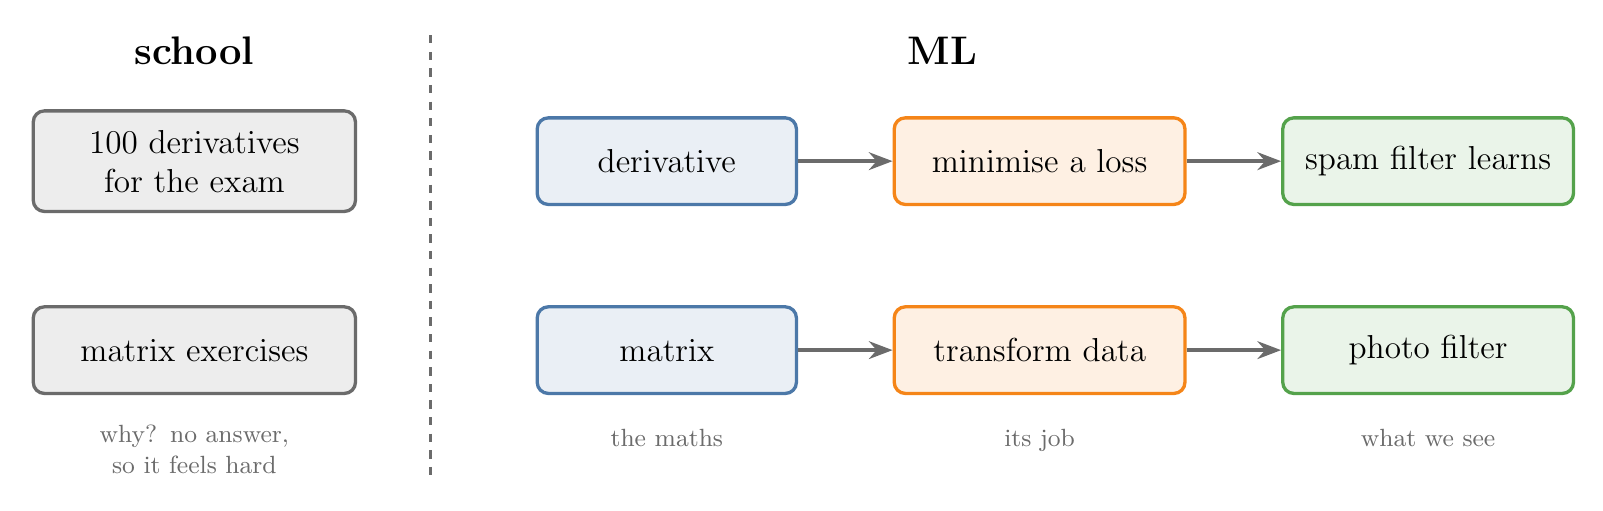
\begin{tikzpicture}[every node/.append style={font=\large}, node distance=1.2cm]
  \node[title] at (0, 1.4) {school};
  \node[title] at (9.5, 1.4) {ML};
  \node[box=cgrey, text width=3.6cm] (s1) at (0, 0) {100 derivatives\\for the exam};
  \node[box=cgrey, text width=3.6cm] (s2) at (0, -2.4) {matrix exercises};
  \node[note, below=0.25cm of s2, text width=4cm] {why? no answer, so it feels hard};
  \node[box=cblue, text width=2.8cm] (d) at (6, 0) {derivative};
  \node[box=corange, text width=3.2cm, right=of d] (dj) {minimise a loss};
  \node[box=cgreen, text width=3.2cm, right=of dj] (de) {spam filter learns};
  \node[box=cblue, text width=2.8cm] (m) at (6, -2.4) {matrix};
  \node[box=corange, text width=3.2cm, right=of m] (mj) {transform data};
  \node[box=cgreen, text width=3.2cm, right=of mj] (me) {photo filter};
  \draw[arrow] (d) -- (dj); \draw[arrow] (dj) -- (de);
  \draw[arrow] (m) -- (mj); \draw[arrow] (mj) -- (me);
  \node[note, below=0.3cm of m] {the maths}; \node[note, below=0.3cm of mj] {its job}; \node[note, below=0.3cm of me] {what we see};
  \draw[cgrey, dashed] (3, 1.6) -- (3, -4);
\end{tikzpicture}
\end{document}
